% Verbatim from minor_report/chapters/chapter_4_results.tex lines 1331-1393 (retired report),
% headings demoted by 0 level(s). Do not edit here; edit the source of the numbers.

Table~\ref{tab:capacity-results} summarizes process-local measurements over the
12 dynamic runs in each requested mode. CPU is the change in cumulative process
CPU time divided by monotonic wall time; 100\% denotes one fully used logical
core, so values above 100\% represent multithreaded execution. Memory is peak
resident set size. The separate detector process, rosbag, Gazebo, RViz, and
RTAB-Map are not included.

\begin{table}[htbp]
\centering
\caption[Dynamic-run capacity and resource measurements, mean $\pm$ sample SD, $n=12$ per row.]{Dynamic-run capacity and resource measurements, mean $\pm$ sample SD,
$n=12$ per row. Nominal VINS+YOLO values are not active-filter measurements.}
\label{tab:capacity-results}
\resizebox{\textwidth}{!}{%
\begin{tabular}{lrrrr}
\toprule
Requested mode & Throughput (Hz) & Retained input (\%) & CPU (\% core) & Peak RSS (MiB) \\
\midrule
VINS-Fusion & $27.14\pm5.81$ & $100.00\pm0.00$ & $443.66\pm58.96$ & $629.51\pm282.62$ \\
ORB-SLAM3 & $23.47\pm4.77$ & $88.55\pm13.42$ & $385.22\pm27.71$ & $1226.06\pm81.83$ \\
VINS-Fusion+YOLO$^{*}$ & $28.83\pm3.16$ & $100.00\pm0.00$ & $406.43\pm89.95$ & $646.14\pm306.15$ \\
ORB-SLAM3+YOLO & $14.47\pm5.42$ & $66.96\pm15.26$ & $410.86\pm42.83$ & $1054.64\pm91.11$ \\
\bottomrule
\multicolumn{5}{l}{$^{*}$Filter requested but no detection frame was matched.}
\end{tabular}}
\end{table}

The ORB+YOLO folders show lower achieved throughput and retention than baseline
ORB, while process CPU is of similar order. This is an observation, not an
isolated detector-cost effect: the external detector is excluded from CPU and 11
paired runs received materially different image counts. Baseline VINS processed
all enqueued images in its logs, whereas baseline ORB discarded frames whenever
the one-frame queue was overwritten.

\begin{figure}[htbp]
  \centering
  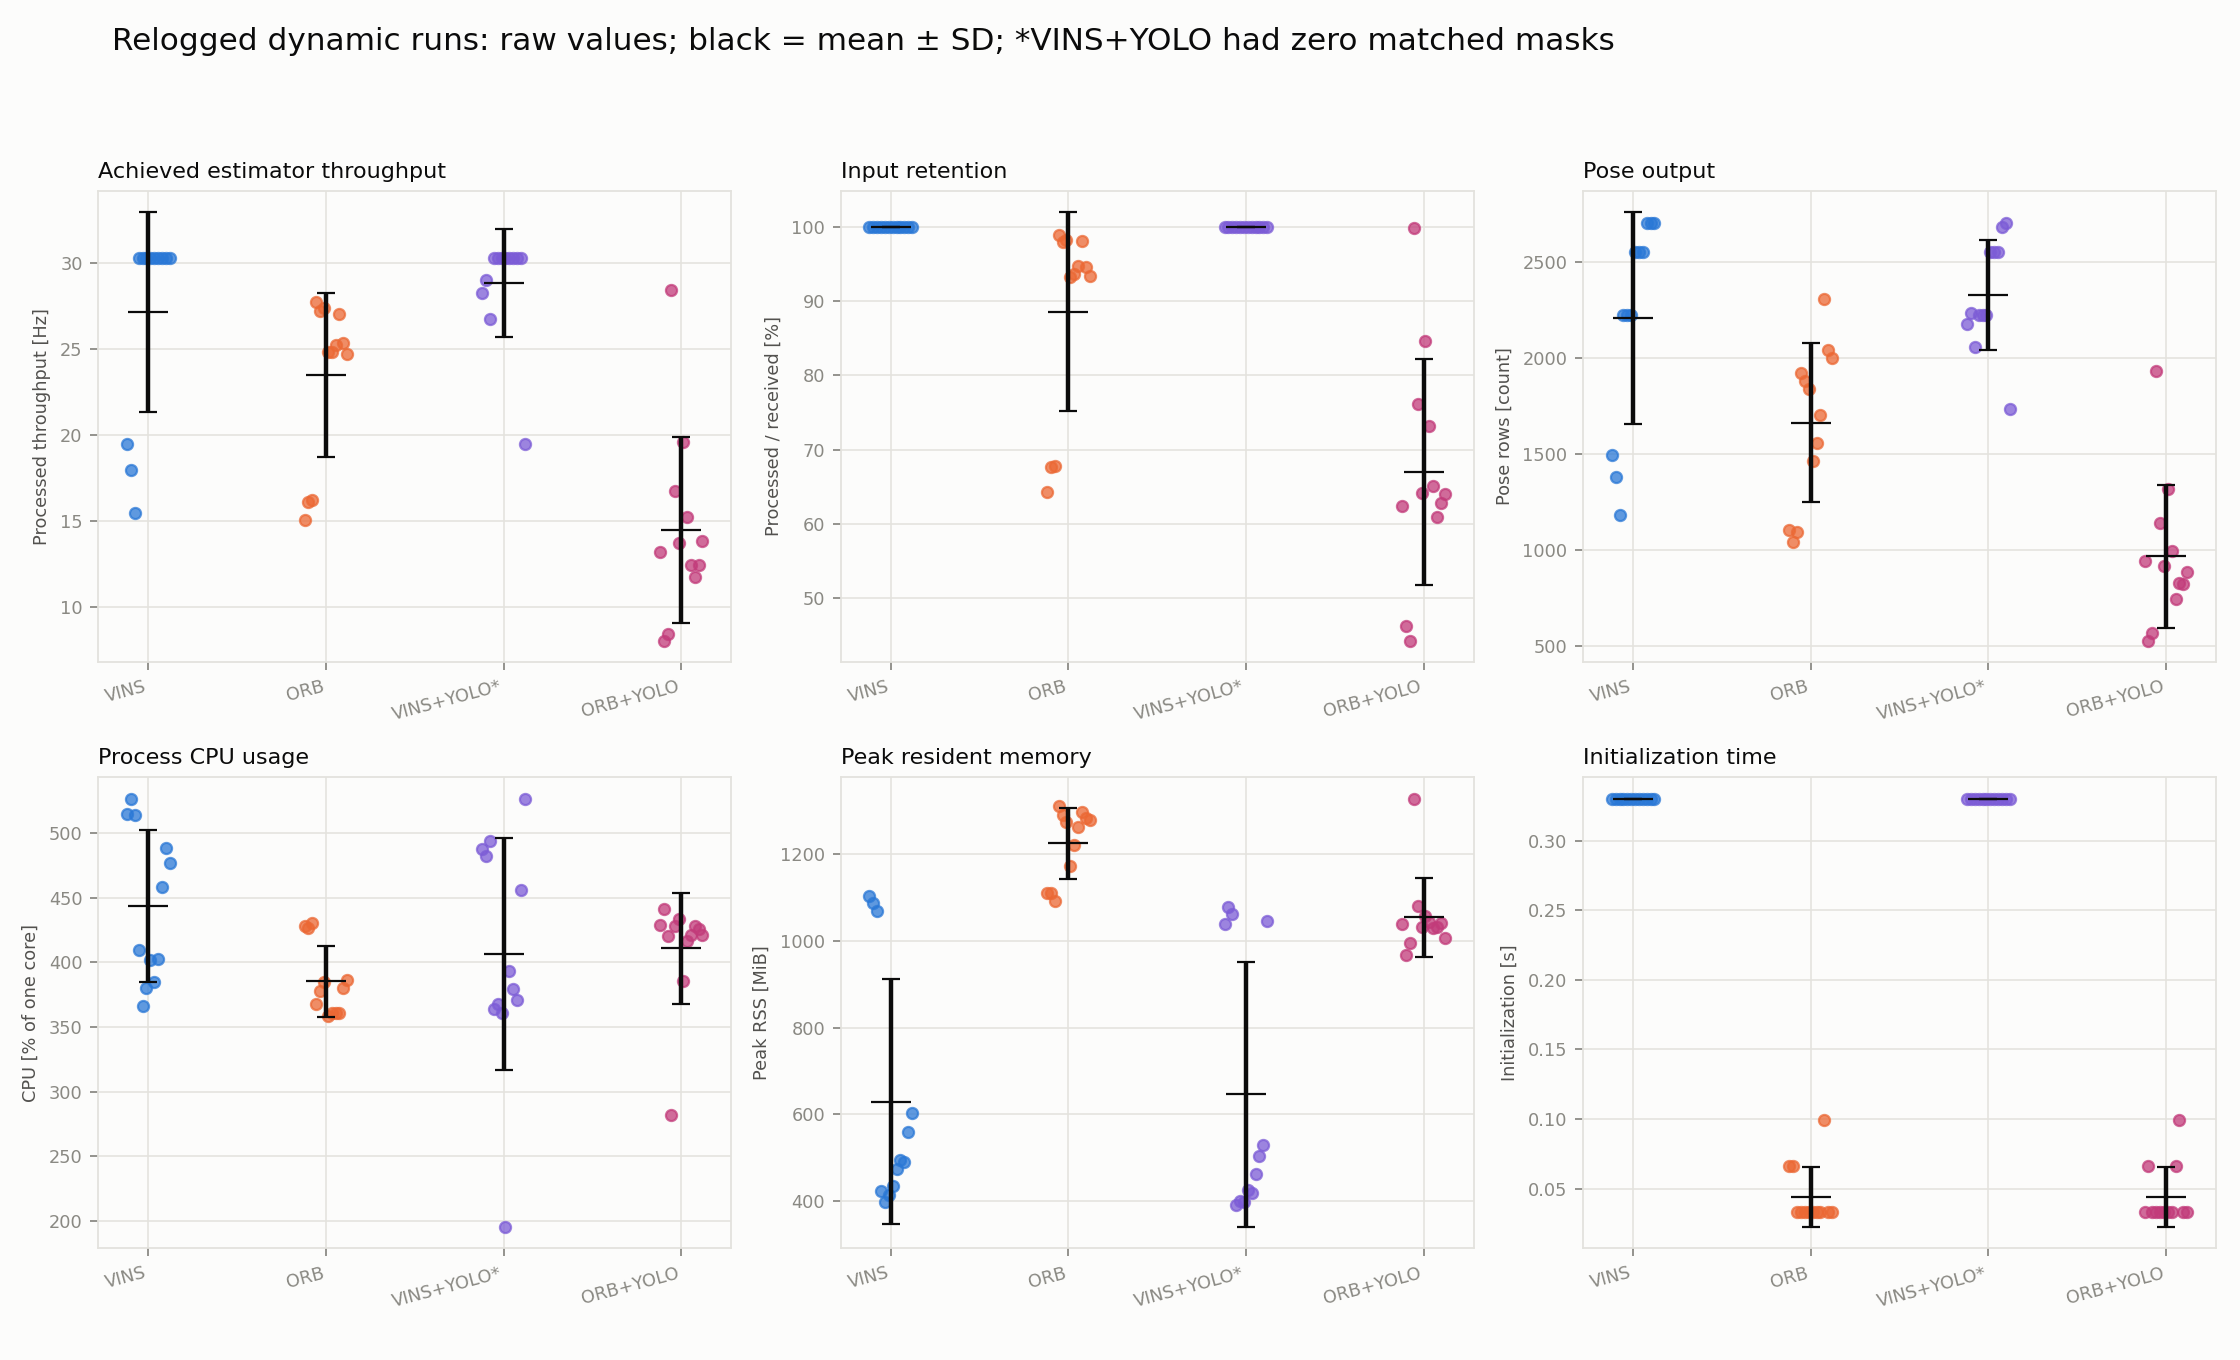
\includegraphics[width=\textwidth]{../../../output/compare/relogged_20260916/capacity_resources_light.png}
  \caption[Raw dynamic-run capacity and process-resource values.]{Raw dynamic-run capacity and process-resource values. Each point is a
  run; black marks show mean $\pm$ sample SD. This plot exposes run-to-run spread
  rather than presenting only aggregate bars.}
  \label{fig:capacity-resources}
\end{figure}

Per-module results use each run's event distribution. Figure~\ref{fig:module-latency}
shows pooled event boxplots for shape, overlaid with one median point per run so
frames are not mistaken for independent experimental repeats. Across run medians,
ORB tracking was $63.19\pm7.06$~ms and ORB local mapping was
$189.58\pm16.95$~ms. The requested ORB+YOLO mode measured
$112.53\pm24.61$~ms and $356.30\pm68.36$~ms respectively. VINS feature tracking
was $48.00\pm10.83$~ms and its back end was $60.41\pm17.12$~ms; nominal
VINS+YOLO values were $43.61\pm11.49$~ms and $57.90\pm16.29$~ms, but cannot be
interpreted as filter effects because that filter was inactive. These timings
refer to different estimator stages and are not added or treated as directly
equivalent algorithms.

\begin{figure}[htbp]
  \centering
  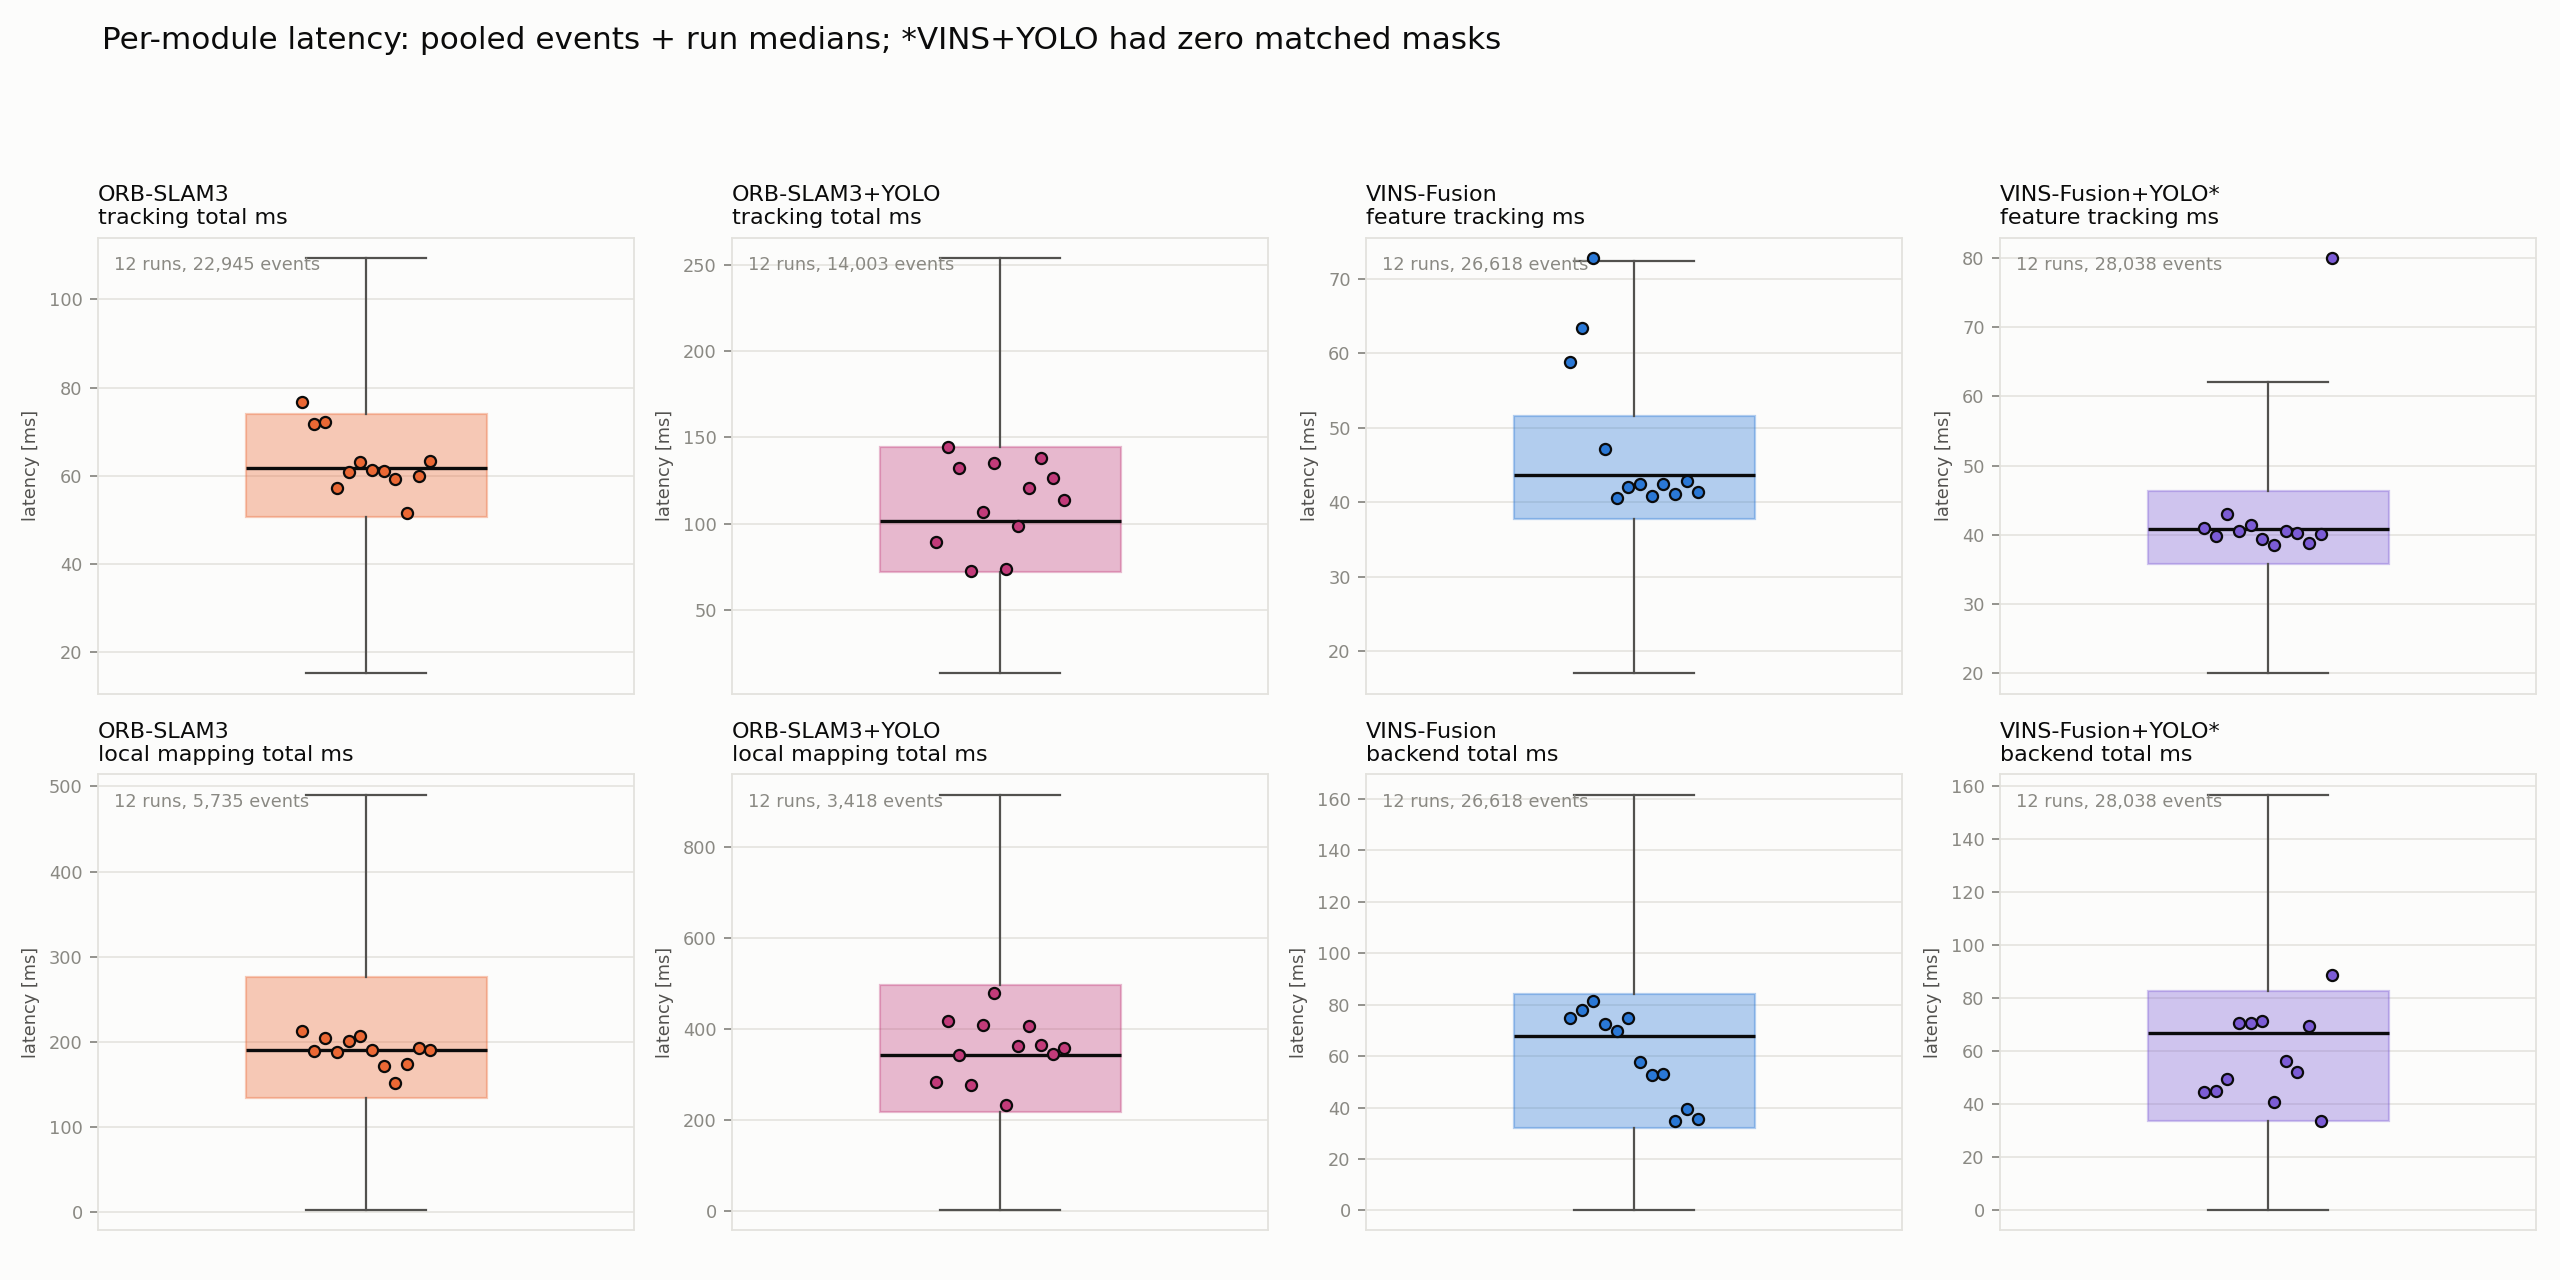
\includegraphics[width=\textwidth]{../../../output/compare/relogged_20260916/module_latency_light.png}
  \caption[Module-latency distributions for dynamic datasets.]{Module-latency distributions for dynamic datasets. Boxes summarize
  all recorded module events; coloured points are per-run medians ($n=12$ in
  each requested mode). ORB local mapping is asynchronous per keyframe, while
  VINS back-end rows follow estimator updates.}
  \label{fig:module-latency}
\end{figure}
